\chapter{The Standard Model and Beyond}\label{ch:theory}

\newcommand{\ct}{\cos\theta_w}
\newcommand{\st}{\sin\theta_w}

In this chapter, we will provide some of the theoretical background that our research builds upon. We will first provide a lightning-quick review of the particle content and gauge structure of the Standard Model, followed by an introduction to Two-Higgs Doublet Models and the Minimal Supersymmetric Standard Model. For excellent treatments of the Standard Model, please see \citep{Cheng:1984,Schwartz:2014,Zee:2003mt,Peskin:1995ev}. For a detailed review of Two-Higgs Doublet Models, see  \cite{Branco:2011iw}, and for a pedagogical introduction to supersymmetry and the MSSM, see \cite{Martin:1997ns}. Our discussion is adapted from these works. 

\section{The Standard Model}\label{sec:sm}

The fundamental constituents of matter are fermions. The interactions between these fermions are mediated by particles known as \emph{gauge bosons}, which arise from the gauge structure of the Standard Model:
\[SU(3)\times SU(2)\times U(1)_Y\]
This means that each fermion transforms in a unique way under transformations corresponding to these gauge groups. In addition to the fermions and gauge bosons, the standard model contains a scalar $SU(2)$ doublet \emph{H}, known as the Higgs field. In \autoref{tab:SM_fields}, we collect the fundamental fields of the SM and their transformation properties under different gauge groups. The labels \emph{u,d,e} and $\nu$ are collective labels for three generations of fermions, shown in \autoref{tab:fermion_generations}. The fields \emph{g}, $W_\mu$, and $B_\mu$ are vector bosons that that correspond to the $SU(3)$, $SU(2)$ and $U(1)$ gauge group respectively.

\begin{table}
  \begin{sidecaption}{The fields of the Standard Model, grouped by their charges under the relevant gauge groups.}[tab:SM_fields]
  \[
  \begin{array}{lccccc}
    \toprule
   \text{Type}                & \text{Field}              & \text{Spin}      & SU(3)      & SU(2)      & U(1)_Y \\\midrule
   \text{Scalar}              & H                         & 0                & \mathbf{1} & \mathbf{2} & \slantfrac{1}{2}\\\midrule
   \text{Fermions}            & Q = \vdoublet{u_L}{d_L}   & \slantfrac{1}{2} & \mathbf{3} & \mathbf{2} & \slantfrac{1}{6}\\
                              & u_R                       &                  & \mathbf{3} & \mathbf{1} & \slantfrac{2}{3}\\
                              & d_R                       &                  & \mathbf{3} & \mathbf{1} & -\slantfrac{1}{3}\\
                              & L = \vdoublet{e_L}{\nu_L} &                  & \mathbf{1} & \mathbf{2} & -\slantfrac{1}{2}\\
                              & e_R                       &                  & \mathbf{1} & \mathbf{1} & -1\\\midrule
    \text{Vector bosons}      & g                         & 1                & \mathbf{8} & \mathbf{1} & 0 \\
                              & W_\mu                     &                  & \mathbf{1} & \mathbf{3} & 0 \\
                              & B_\mu                     &                  & \mathbf{1} & \mathbf{1} & 0\\
    \bottomrule
  \end{array}
\]
\end{sidecaption}
\end{table}

The ground state that we inhabit spontaneously breaks the larger symmetry $SU(2)\times U(1)_Y$ to the symmetry $U(1)_\text{EM}$. The subscript \emph{Y} denotes the hypercharge of the field, while the subscript EM denotes electromagnetism. In this process (which we will revisit in more detail in \autoref{subsec:ewsb}), the three gauge fields $W_\mu$, corresponding to the $SU(2)$ gauge symmetry, combine with the $B_\mu$ field corresponding to the $U(1)_Y$ symmetry to form the massive gauge bosons $W^\pm$ and $Z$, and a massless photon, $A_\mu$ (often denoted by $\gamma$ instead). The \emph{W} and \emph{Z} bosons mediate the weak interactions that responsible to phenomena such as radioactive decay, while the photon mediates electromagnetic interactions. The gauge field \emph{g} corresponding to the $SU(3)$ gauge symmetry is known as the \emph{gluon}, and mediates the strong force between nucleons. 


\begin{table}
  \raggedright
\strictpagecheck
\begin{adjustwidth}{-0.5in}{0in}
  \begin{tabular}{cllll}
    \toprule
    Generation & \multicolumn{2}{c}{Quarks} & $e$: Leptons & $\nu$: Neutrinos \\ \cmidrule(r){2-3}
     & $u$: Up & $d$: Down &                                       & \\\midrule
    I           & $u:$ up                    & $d:$ down     & $e:$ electron                         & $\nu_e:$ electron neutrino\\
    II          & $c:$ charm                 & $s:$ strange  & $\mu:$ muon                           & $\nu_\mu:$ muon neutrino\\
    III         & $t:$ top                   & $b:$ bottom   & $\tau:$ tau                           & $\nu_\tau:$ tau neutrino\\
    \bottomrule
  \end{tabular}
  \caption{The fermion sector of the Standard Model, grouped by generation.}
  \label{tab:fermion_generations}
\end{adjustwidth}
\end{table}
\subsection{Electroweak symmetry breaking}\label{subsec:ewsb}
In 1957, Schwinger proposed the unification of the weak and electromagnetic interactions, citing their vectorial nature. In 1961, Glashow proposed a model for weak interactions governed by symmetry under the product group $SU(2)\times U(1)$. The trouble was, experiments had shown that the weak interactions had a short range, implying that the vector bosons that mediated them must be massive. On the other hand, gauge symmetry prohibits mass terms for these intermediate vector bosons. Glashow's theory included these mass terms, but they were put in by hand, and spoiled the renormalizability of the theory. A possible way out was to break the gauge symmetry \emph{spontaneously} rather than explicitly. Spontaneous symmetry breaking refers to the phenomenon where the ground state of a system does not respect the symmetry of the full Lagrangian. However, Goldstone's theorem states that for every spontaneously broken symmetry, there exists a set of massless spin-0 bosons corresponding to the generators of the symmetry group - since such particles have never been observed, this was obviously an undesirable feature of the theory. 

Thus we seem to have to choose between two undesirable outcomes: a set of massless gauge bosons, or a set of massless scalars, both of which are inconsistent with what we actually see in nature. Remarkably, each of these problems would turn out to be the solution for the other, through the marvelous \emph{Higgs mechanism}. This mechanism was first put forth by Philip W. Anderson in the context of condensed matter systems. In 1964, three groups -- Peter Higgs, the duo of Francois Englert and Robert Brout, and the trio of Gerald Guralnik, C. R. Hagen, and Tom Kibble -- independently and almost simultaneously proposed that this mechanism could explain how the the weak interaction mediators can acquire mass. There is likely a strong case for naming the mechanism after all of these physicists, but for the sake of expediency, we will simply refer to it as the Higgs mechanism.

The Higgs mechanism describes the spontaneous breaking of electroweak symmetry, that is, the breakdown of the product group $SU(2)\times U(1)_Y\rightarrow U(1)_{EM}$. This is achieved by adding to the theory a complex scalar $SU(2)$ doublet, the Higgs field $H$:
\[H = \vdoublet{H^+}{H^0}.\]
The terms of the Lagrangian that involve this field can be written as follows:
\begin{align}
  \label{eq:higgs_kinetic}
  \mathcal{L}_{\text{Higgs}} &= \frac{1}{2}\left|D_\mu H\right|^2-V(H)\\
  \label{eq:higgs_potential}
  \text{where }V(H) &= \left(H^\dag H-\frac{v^2}{2}\right)^2
\end{align}
The gauge covariant derivative for the Standard Model takes the form (neglecting the term corresponding to the unbroken $SU(3)$ symmetry)
$$D_\mu = \partial_\mu + igW_\mu^aT^a+ig'YB_\mu,$$
where $W_\mu^a$ and $B_\mu$ are the gauge fields corresponding to the $SU(2)$ and $U(1)_Y$ symmetries respectively, \emph{g} and $g'$ are coupling constants, and $T^a$ and $Y$ are the generators of the $SU(2)$ and $U(1)$ groups. The potential $V(H)$ reaches its minimum when $H^\dag H = v^2 / 2$. We pick a non-zero vacuum expectation value (VEV) for $H$ that breaks the neutral sector symmetry (corresponding to $H^0$) but not the charged symmetry (corresponding to $H^{+}$), since we wish to keep photons massless. This VEV is given by:
\[H = \vdoublet{0}{\frac{v}{\sqrt{2}}}.\]
Plugging this into the kinetic term of the Lagrangian, and isolating the terms quadratic in the gauge fields, we get
\[\frac{g^2v^2}{4}W_\mu^-W_\mu^++\frac{1}{2}\frac{v^2}{4}(g^2+g'^2)
\left(\ct W_\mu^3 - \st B_\mu\right)^2\]
where $W_\mu^\pm = (W_\mu^1\pm iW_\mu^2)/\sqrt{2}$  and $\theta_w = \tan^{-1}(g'/g)$ is the \emph{Weinberg angle}, which parameterizes the mixing between the photon $A_\mu$ and the $Z$ boson $Z_\mu$.
\begin{equation}\label{eq:z_a_mixing}
\vdoublet{Z_\mu}{A_\mu} = \fourmatrix{\ct}{-\st}{\st}{\ct}
\vdoublet{W_{\mu}^{3}}{B_{\mu}}
\end{equation}
The product $W_\mu^+W_\mu^-$ can be interpreted as a mass term for a charged vector boson, $W_\mu^\pm$. Collecting the terms quadratic in $W_\mu^\pm$ and $Z_\mu$, we get
\[\mathcal{L}_{\text{mass terms}}=\frac{e^2v^2}{4\sin^2\theta_w}W_\mu W^\mu+
\frac{e^2v^2}{8\sin^2\theta_w\cos^2\theta_w}Z_\mu Z^\mu.\]
Thus, after accounting for symmetry factors, we get the masses of the \emph{W} and \emph{Z} bosons as:
\begin{align*}
  m_W &=\frac{ev}{2\st}, & 
  m_Z &=\frac{ev}{\sin2\theta_w}.
\end{align*}
We see that there is no mass term for $A_\mu$. Thus the \emph{W} and \emph{Z} bosons gain mass, limiting their range, while the photon remains massless, corresponding to what is experimentally observed. Remarkably, we have done this without violating gauge invariance. Colloquially, we say that the \emph{W} and \emph{Z} bosons have `eaten' the Goldstone boson degrees of freedom to obtain mass. 

Peter Higgs was the first to postulate the existence of a physical scalar particle that could be produced by perturbing the vacuum. To see how this plays out, let us parameterize the Higgs doublet field as 
\[H = \frac{1}{\sqrt{2}}\exp\left(i\xi^a(x)\frac{\tau^a}{v}\right)\vdoublet{0}{v + h(x)}.\]
where $\tau^a$ are the Pauli matrices, $\xi^a$ and $h$ are scalar fields with VEVs given by $\langle\xi\rangle=\langle h\rangle=0$, and \emph{v} is the vacuum expectation value of the Higgs doublet, experimentally measured to be about 246 GeV. The field $h$ is known as the \emph{Higgs boson}. The simplest gauge choice to examine this scenario is the unitary gauge, where $\xi(x)=0$. In this gauge, the potential $V(H)$ from \eqref{eq:higgs_potential} becomes:
\[V(H) = -\frac{1}{2}m_h^2 h^2 - \lambda vh^3 -\frac{1}{4}\lambda h^4\]
The Higgs boson is the only fundamental scalar in the Standard Model, and was discovered in 2012, nearly 50 years after it was first predicted. The coefficient of the term quadratic in $h$ is its mass, $m_h$ - a free parameter that had to be determined experimentally. The second and third terms in the above expression represent the trilinear and and quartic self-coupling of the Higgs boson.
\subsection{Quark mass and gauge eigenstates}
While the quarks listed in \autoref{tab:fermion_generations} are \emph{gauge eigenstates}, with well defined transformations under the gauge groups, the physical states that we observe at a collider will in fact be \emph{mass eigenstates}. The two are related by the \emph{Cabibbo-Kobayashi-Maskawa} (\textsc{ckm}) matrix:
\sidepar{The Cabibbo-Kobayashi-Maskawa quark mixing matrix}
\begin{equation}
  V_\text{CKM} =
  \begin{pmatrix}
    V_{ud} & V_{us} & V_{ub}\\
    V_{cd} & V_{cs} & V_{cb}\\
    V_{td} & V_{ts} & V_{tb}
  \end{pmatrix}
\end{equation}
The elements of the matrix denote the level of mixing between the gauge eigenstates. Experimentally, this matrix has been determined to be nearly diagonal.

\subsection{Asymptotic freedom and QCD}

In the 50s and 60s, experiments were devised to unravel the structure of the proton. They found two seemingly incompatible results. On the one hand, colliding protons resulted in the production of a large number of pions collinear with the beam axis, implying that the protons could not absorb a large momentum transfer. However, deep inelastic scattering experiments later showed that it was possible for an energetic electron to undergo hard electromagnetic scattering off a proton. These disparate phenomena were reconciled by the introduction of the \emph{parton model} by Bjorken and Feynman. In this model, hadrons such as the proton were comprised of a collection of loosely bound pieces, known as partons (for an artistic representation, see \autoref{fig:proton_innards}). To an energetic incoming electron, these partons would appear approximately free, allowing it to scatter with a large momentum transfer off of one of them. The struck parton will then exchange momentum softly via the strong interaction among the other partons, which results in the production of a \emph{jet} of hadrons, collinear with the direction of the original struck parton. The deeper reason for this behavior is that these partons are charged under a non-Abelian gauge group, $SU(3)$. The phenomenon of the weakening of the interaction strength at large momentum transfers is known as \emph{asymptotic freedom}, and it is a property of non-Abelian gauge theories.
\begin{marginfigure}[-3in]
  \strictpagecheck
  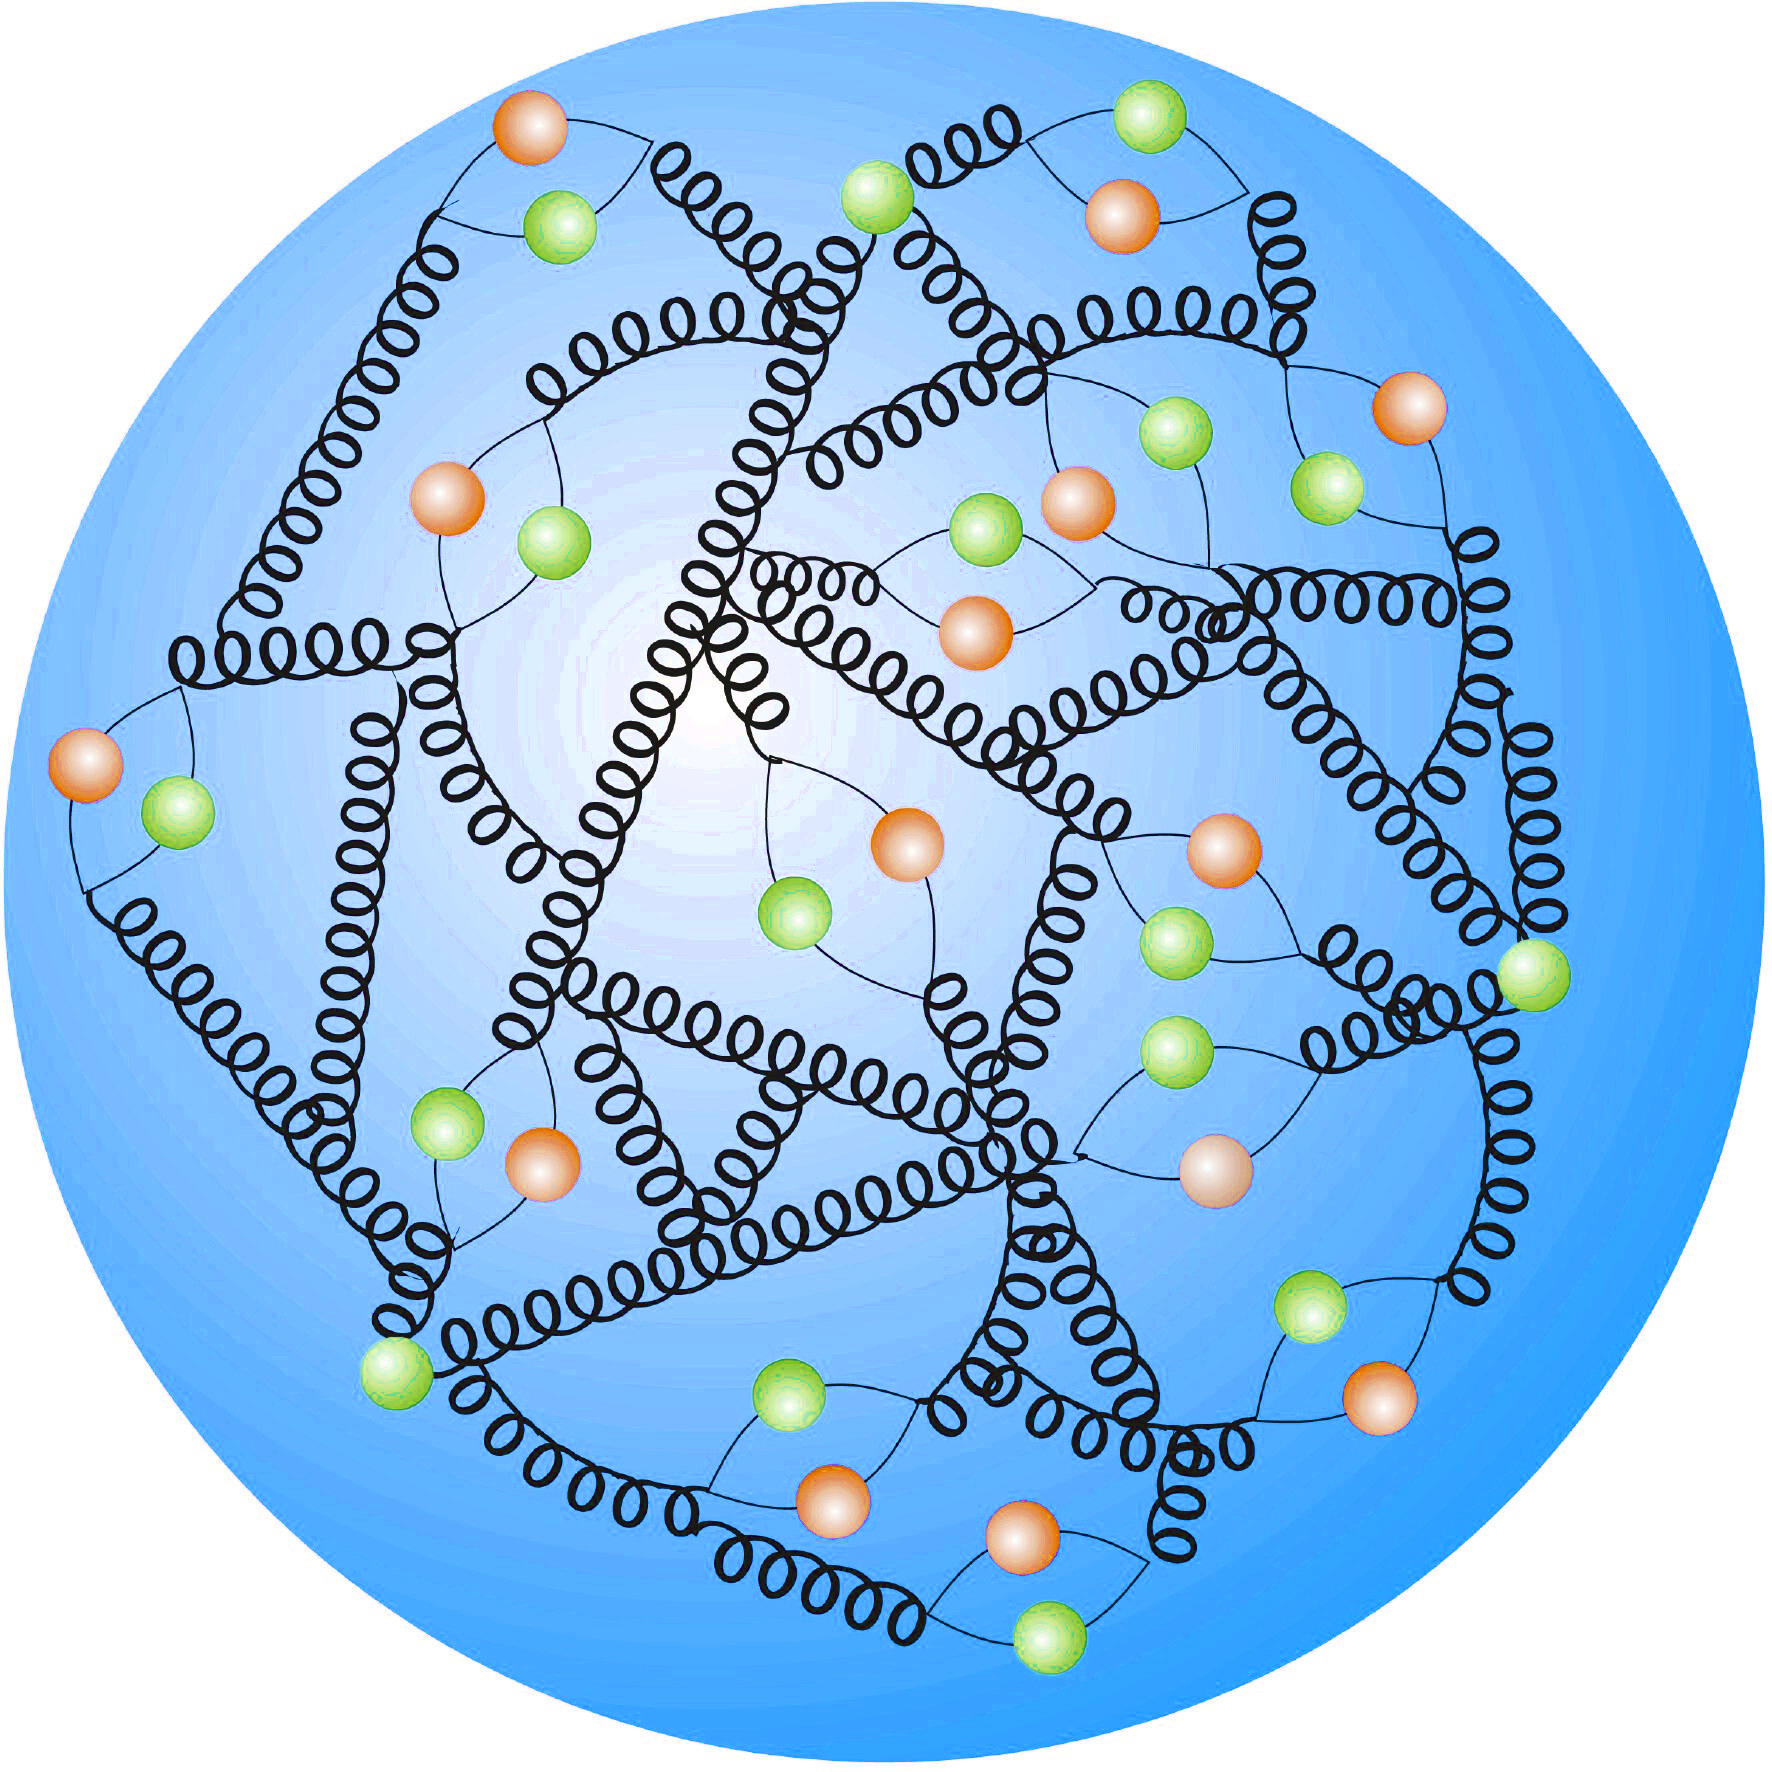
\includegraphics[width=0.8\textwidth]{images/proton_innards}
\caption{A representation of the innards of a proton, showing the dynamic structure. Source: \citep{proton_structure}}
\label{fig:proton_innards}
\end{marginfigure}
The $\beta$-function of a gauge theory describes the evolution of the renormalized coupling constant with energy. For non-Abelian gauge theories, it takes the following form (up to leading order):%
\sidepar{Leading order $\beta$-function for non-Abelian gauge theories}
\begin{equation}
  \beta(g_R) = \mu\frac{d}{d\mu}g_R = -\frac{g_R^3}{(4\pi)^2}\left[\frac{11}{3}C_A -\frac{4}{3}n_fT_F\right]
\end{equation}
where $\mu$ is the renormalization scale, $C_A$ is the quadratic Casimir operator for the adjoint representation, and $T_F$ is the \emph{index} of the fundamental representation.
In the case of the strong interaction, the relevant gauge group is $SU(3)$. Thus $C_A = 3$ and $T_F = \frac{1}{2}$. If $n_f$, the number of quark flavors is less than 17 \footnote{Which it is, since the number of quark flavors is six, as can be seen in \autoref{tab:fermion_generations}.}, the $\beta$ function has a \emph{negative} sign, which means that the coupling \emph{decreases} at higher energies. This is the underlying basis of asymptotic freedom. The theory of the strong interaction is known as \emph{quantum chromodynamics}, or QCD for short. The analogue of electric charge for this theory is a quantity referred to as \emph{color} (hence the name of the theory). At a hadron collider, it is of crucial importance to understand the physics of gluons and jets.

The Standard Model of particle physics has been remarkably successful, and over the decades has yielded some of the most precise measurements in all of physics. However, as mentioned in \autoref{ch:introduction}, there still remain unresolved issues with it. In the next two sections we will discuss some of these issues in more depth, and introduce extensions to the SM that potentially resolve them.

\section{Two-Higgs Doublet Models}\label{sec:2HDMs}

Intuitively, it is not too hard to imagine, based on the complex structure of the fermion and gauge sectors of the Standard Model, that its scalar sector might well contain members other than a single $SU(2)$ doublet. An extended scalar sector frequently arises in BSM theories that potentially alleviate some of the unresolved issues facing the Standard Model.
% Strong CP problem
One of these issues is the \emph{strong CP problem}, which can be summarized as follows. Lagrangians for Yang-Mills theories can have a renormalizable term that is gauge-invariant but violates CP, of the form
\[\mathcal{L}_{\theta} = \theta\epsilon^{\mu\nu\alpha\beta}F_{\mu\nu}^aF_{\alpha\beta}^a,\]
where $\theta$ is some angle, $F_{\mu\nu}^a$ are the field strength tensors, and $\epsilon^{\mu\nu\alpha\beta}$ is an antisymmetric tensor. This term is a total derivative, since it can be written as $2\theta\partial_\mu(\epsilon^{\mu\nu\alpha\beta}A_\nu^aF_{\alpha\beta}^a)$. Thus, it should not contribute to perturbative effects. However, this term can potentially contribute to non-perturbative effects. Additionally, this term can be modified be chiral rotations of the form $\psi\rightarrow \exp(i\gamma_5\theta_F)\psi$. Since physical observables should be independent of the choice of the basis, i.e. $\theta_F$, we should absorb it into $\theta$ by defining a basis-independent phase: $\bar{\theta} = \theta-\theta_F$. For $SU(2)$ and $U(1)$ gauge symmetries, this phase can be set to zero by performing appropriate chiral rotations of the fermion fields. However, no such choice exists for the term corresponding to the the $SU(3)$ group, and thus the CP-violating term in the QCD Lagrangian could in principle by non-zero. A non-zero value of $\bar{\theta}$ would be manifested as non-perturbative effects. For example, the neutron would then have a non-zero electric dipole moment. However, experiments have shown that $\bar{\theta}$ must be vanishingly small, with a stringent upper bound: $\bar{\theta}<10^{-10}$. A value this small seems suspiciously \emph{fine-tuned} in the absence of an underlying symmetry to enforce it.

Adding an additional scalar doublet allows us to impose such a symmetry - a global $U(1)$ symmetry known as \emph{Peccei-Quinn} symmetry. If this symmetry is spontaneously broken, a Goldstone boson arises, which can then be chirally rotated such that $\bar{\theta}$ becomes effectively zero for the ground state.
% Baryon asymmetry
Extended scalar sectors also arise in theories that can explain the observed imbalance between matter and antimatter in the universe. The CP violation in the weak sector of the Standard Model cannot account for this imbalance, but $2$HDMs, with their complex scalar sector and possible new sources of CP violation, can.
%
However, the strongest motivation for $2$HDMs is their connection to supersymmetric models that have the potential to resolve the hierarchy problem, discussed in the next section. The scalar sector of the Minimal Supersymmetric Standard Model  has a structure similar to that of a $2$HDM - it requires exactly two scalar doublets to give mass to both up and down type fermions, and for the cancellation of anomalies. With these motivations for $2$HDMs in mind, let us examine the structure of the scalar potential of a generic Two-Higgs Doublet Model.

\subsection{The $2$HDM scalar potential}
The most general renormalizable scalar potential for two scalar doublets $\Phi_1$ and $\Phi_2$ with hypercharge $+1$ is given by
\strictpagecheck
\sidepar{Scalar potential for a Two-Higgs Doublet Model}
\begin{align}
\label{eq:2HDM_scalar_potential}
  \begin{split}
  V(\Phi_1,\Phi_2) &= m_{11}^2|\Phi_1|^2 + m_{22}^2|\Phi_2|^2 - m_{12}^2\left(\Phi_1^\dagger\Phi_2 + \text{h.c.}\right)\\
&+\frac{\lambda_1}{2}|\Phi_1|^4 + \frac{\lambda_2}{2}|\Phi_2|^4+\lambda_3|\Phi_1|^2|\Phi_2|^2 + \lambda_4|\Phi_1^\dagger\Phi_2|^2\\
&+\left[\frac{\lambda_5}{2}\left(\Phi_1^\dagger\Phi_2 \right)^2+\lambda_6|\Phi_1|^2(\Phi_1^\dagger\Phi_2)+\lambda_7|\Phi_2|^2(\Phi_1^\dagger\Phi_2) + \text{h.c.}\right]
\end{split}
\end{align}
where h.c. stands for the hermitian conjugate of the terms immediately preceding it. The parameters $m_{11,22}^2$ and $\lambda_{1,2,3,4}$ are real while the parameters $m_{12}^2$ and $\lambda_{5,6,7}$ can be complex. Naively, it would seem that this potential has 14 degrees of freedom - six from the real parameters, and eight from the complex parameters. However, it should be noted that we have the freedom to perform basis transformations, that is, we can write the potential in terms of new doublets $\Phi_a' = \sum_{b=1}^2U_{ab}\Phi_b$. where $U_{ab}$ is a 2$\times$2 unitary matrix. The condition of unitarity implies that $U$ has three degrees of freedom, which can absorb three out of the 14 degrees of freedom listed earlier. Thus, only 11 out of the original 14 degrees of freedom are physical.

In principle, we could proceed with these 11 parameters, however, there are a couple of reasons to attempt to reduce this number. The first is that a large number of free parameters makes a theory less falsifiable, thus reducing its predictive power. The second is that in order to distinguish between pseudoscalars and scalars, CP must be conserved in the Higgs sector. Finally, the potential in \eqref{eq:2HDM_scalar_potential} allows for tree-level flavor-changing neutral currents (FCNC), which are experimentally measured to be highly suppressed. These can be eliminated by introducing discrete or continuous symmetries. Imposing a discrete symmetry such as $\mathcal{Z}_2$\footnote{That is, the Lagrangian is invariant under the reflection of one of the doublets: \[\Phi_i\rightarrow-\Phi_i\].} removes the terms that are odd in $\Phi_i$. This effectively sets $\lambda_6=\lambda_7 = 0$. In principle, this should set $m_{12} = 0$ as well, but we retain this term since it breaks the $\mathcal{Z}_2$ symmetry softly, relaxing the experimental bounds on the mass spectrum.
After imposing these constraints, all the remaining parameters $\lambda_{1,2,3,4,5}, m_{11,12,22}^2$ are real. From here on, we will only consider $2$HDMs with these constraints. 

There are four such models, classified based on the coupling patterns of the fermions to the two Higgs doublets. In Type I $2$HDMs, all the quarks couple to only one of the Higgs doublets, chosen by convention to be $\Phi_2$. In Type II $2$HDMs, the up-type right-handed quarks (\emph{u,c,t}) couple to $\Phi_2$, and the down-type right-handed quarks (\emph{d,s,b}) couple to $\Phi_1$. In both of these models, the right-handed leptons couple to the same doublet as the down-type quarks. The lepton-specific model is similar to the Type I model, except in this case, the right-handed leptons couple to $\Phi_1$. Similarly, the `flipped' model is similar to the Type II $2$HDM, except that the leptons couple to $\Phi_2$. The coupling patterns for these models are collected in \autoref{tab:no_FCNC_$2$HDMs}.
\begin{margintable}[0.5cm]
\small{
  \begin{tabular}{lccc}
	\toprule
    Model & $u_R^i$ & $d_R^i$  & $e_R^i$\\
    \midrule
    Type I          & $\Phi_2$ & $\Phi_2$ & $\Phi_2$\\
    Type II         & $\Phi_2$ & $\Phi_1$ & $\Phi_1$\\
    Lepton-specific & $\Phi_2$ & $\Phi_2$ & $\Phi_1$\\
    Flipped         & $\Phi_2$ & $\Phi_1$ & $\Phi_2$\\
    \bottomrule
  \end{tabular}}
  \caption{Fermion coupling patterns for $2$HDMs with flavor conservation.}
  \label{tab:no_FCNC_$2$HDMs}
\end{margintable}
\noindent The scalar potential $V(\Phi_1,\Phi_2)$ is minimized for non-zero vacuum expectation values of $\Phi_i$:
\begin{align}
\langle\Phi_i\rangle_0=\vdoublet{0}{\frac{v_i}{\sqrt{2}}}.
\end{align}
where $v_i$ are the vacuum expectation values of the doublets $\Phi_i$. These doublets can then be written as follows:
\begin{equation}\label{eq:2HDM_doublet_components}
\Phi_i = \vdoublet{\phi_i^+}{\frac{1}{\sqrt{2}}(v_i+\rho_i+i\eta_i)}
\end{equation}
where $\phi_i^+$ are complex charged scalars, and $\rho_i$ and $\eta_i$ represent the real and complex degrees of freedom of the neutral components of the doublets. The two doublets, each with two complex components, embody eight degrees of freedom in total. 
The process of electroweak symmetry breaking causes three of these degrees of freedom to be `eaten' by the \emph{W} and \emph{Z} bosons, and the remaining five are manifested as physical scalar fields. These consist of a pair of CP-even neutral scalars \emph{h} and \emph{H}, a CP-odd pseudoscalar \emph{A}, and a charged scalar $H^\pm$.

\subsection{The $2$HDM mass spectrum}

In this section, we will analyze the mass spectrum of flavor-conserving $2$HDMs. To do so, we construct the mass matrices by taking derivatives of the scalar potential
\[M_{ij} = \frac{\partial V(\Phi_1,\Phi_2)}{\partial\phi_i\partial\phi_j},\]
where $\phi_{i}$ can be any of the fields $\phi_i^+,\rho_i,\eta_i$ in \eqref{eq:2HDM_doublet_components}. 
Applying this procedure to the charged scalar components $\phi_i^\pm$, we obtain their mass matrix $M_{\phi^{\pm}}$:
\[M_{\phi^\pm} = \left[m_{12}^2-(\lambda_4+\lambda_5)v_1v_2\right]\fourmatrix{v_2/v_1}{-1}{-1}{v_1/v_2}.\]
Diagonalizing this matrix gives us the mass of the charged Higgses:
\[m_{H^\pm}^2 = (v_1^2+v_2^2)\left[m_{12}^2/v_1v_2-(\lambda_4+\lambda_5)\right].\]
Similarly, the mass matrix for the pseudoscalars is given by
\[M_{\eta} = \frac{m_A^2}{v_1^2+v_2^2}\fourmatrix{v_2^2}{-v_1v_2}{-v_1v_2}{v_1^2}.\]
Diagonalizing it gives us a massless Goldstone boson $G^0$, corresponding to a zero eigenvalue, and a pseudoscalar Higgs boson $A$, with mass given by
\[m_A^2 = (v_1^2+v_2^2)\left[m_{12}^2/v_1v_2-2\lambda_5\right].\]
The diagonalization process amounts to a rotation of the basis vectors by some angle. For the CP-odd and the charged scalars, this angle is the same, and is denoted as $\beta$. Given that the couplings of the Higgs bosons in $2$HDMs depend on this angle and the angle $\alpha$ \eqref{eq:alpha_def}, let us adopt the notation 
\[s_\theta,c_\theta,t_\theta = \sin\theta,\cos\theta,\tan\theta\]
for brevity. In this notation, the mass eigenstates are given by
\begin{align}
\vdoublet{A}{G^0} = \fourmatrix{s_\beta}{-c_\beta}{c_\beta}{s_\beta}\vdoublet{\eta_1}{\eta_2}&&\text{and}&&
\vdoublet{H^\pm}{G^\pm} = \fourmatrix{s_\beta}{-c_\beta}{c_\beta}{s_\beta}\vdoublet{\phi_1^+}{\phi_2^+}.
\end{align}
The angle $\beta$ turns out to be a very important one for studying $2$HDMs. It also represents the ratio of the vacuum expectation values of the neutral components of the two Higgs doublets: $t_\beta = v_2/v_1$.
Finally, the mass matrix for the CP-even scalars is given by
\[M_{\rho} = -\fourmatrix{m_{12}^2\frac{v_2}{v_1}+\lambda_1v_1^2}{-m_{12}^2+\lambda_{345}v_1v_2}{-m_{12}^2+\lambda_{345}v_1v_2}{m_{12}^2\frac{v_2}{v_1}+\lambda_1v_2^2},\]
where $\lambda_{345} = \lambda_3+\lambda_4+\lambda_5$. This matrix is diagonalized by rotation of the basis vectors by the angle $\alpha$:
\begin{equation}
\vdoublet{h}{H} = \fourmatrix{s_\alpha}{-c_\alpha}{-c_\alpha}{-s_\alpha}\vdoublet{\rho_1}{\rho_2}.
\label{eq:alpha_def}
\end{equation}
The mass eigenstates are labeled $h$ and $H$, with $h$ traditionally taken to be the lighter of the two.

%\begin{align}
%v &= v_1^2 + v_2^2
%\end{align}
Thus we see that the physical spectrum of $2$HDMs contains five mass eigenstates: the CP-even higgses $h$ and $H$, the CP-odd pseudoscalar Higgs $A$, and a pair of charged Higgses $H^\pm$. Incidentally, the Standard Model Higgs is taken to be a combination of the CP-even Higgses:
\begin{equation}
  h_\text{SM} = \rho_1c_\beta + \rho_2s_\beta = hs_{\alpha-\beta}-Hc_{\alpha-\beta}.
\label{eq:h_SM}
\end{equation}

\subsection{$2$HDM Interactions}

\newcommand{\sbma}{s_{\beta-\alpha}}
\newcommand{\cbma}{c_{\beta-\alpha}}
\newcommand{\casb}{c_\alpha/s_\beta}
\newcommand{\sacb}{s_\alpha/c_\beta}
\newcommand{\sasb}{s_\alpha/s_\beta}

In this section, we discuss the $2$HDM interactions that are relevant to our analyses, namely, the ones governing the exotic decays of Higgses to other, lighter Higgses, and the subsequent decays of the lighter Higgses to SM fermions. The decays to SM fermions are governed by the Yukawa terms in the Lagrangian:
\sidepar{Yukawa interactions}
\begin{align*}
&\mathcal{L}^{\mathrm{2HDM}}_{\text{Yukawa}} = - \sum_{f = u, d, l} \frac{m_f}{v}
\left(\xi_h^f \overline{f}fh+\xi_H^f \overline{f}fH-i\xi_A^f \overline{f}\gamma_5fA \right)\\
&-\left\{\frac{\sqrt{2}V_{ud}}{v}\overline{u}\left(m_u\xi_A^uP_l+m_d\xi_A^dP_R\right)dH^+ + \frac{\sqrt{2}m_l\xi^l_A}{v}\overline{\nu}_Ll_RH^+ + h.c.\right\}
\label{eq:2HDM_Yukawa_couplings}
\end{align*}
where $f$ is a fermion with mass $m_f$, the fields $u$ and $d$ are up and down type quarks with masses $m_u$ and $m_d$ and CKM mixing $V_{ud}$, $l$ is a lepton with mass $m_l$, and $\nu_L$ is a neutrino. 
The factors $\xi$ in the above expressions depend on the specific model being considered. For the Type II $2$HDM, they take the values listed in \autoref{tab:xi_factors}.
\begin{margintable}[2in]
  \[
    \begin{array}{lr}
      \toprule
      \text{Coefficient}       & \text{Value} \\
      \midrule
      \xi_{h}^u   & \casb          \\
      \xi_{h}^d   & -\sacb         \\
      \xi_{h}^l   & -\sacb         \\
      \xi_{H}^u   & \sasb          \\
      \xi_{H}^d   & \casb          \\
      \xi_{H}^l   & \casb          \\
      \xi_{A}^u   & 1/t_\beta      \\
      \xi_{A}^d   & t_\beta        \\
      \xi_{A}^l   & t_\beta\\      
      \bottomrule
\end{array}
\]
\caption{The factors $\xi$ that determine the Yukawa couplings of Higgs bosons in Type II $2$HDMs.}
\label{tab:xi_factors}
\end{margintable}

For the exotic decays, we can obtain the coupling strengths from the kinetic terms for the fields $\Phi_i$, similar to what we do for the SM electroweak interactions. With a little bit of work, we can extract the following couplings (see \citep{Kling:2016yls} for details):
\begin{align*}
& g_{AH^\pm W^\mp} & = && \frac{g}{2}(p_{H^+}-p_{A})^\mu\\
& g_{hAZ}          & = && is_{\beta-\alpha}\frac{g}{2c_{\theta_w}}(p_A-p_h)^\mu\\
& g_{hH^\pm W^\mp} & = && -is_{\beta-\alpha}\frac{g}{2}(p_{H^\pm}-p_h)^\mu\\
& g_{HAZ}          & = && ic_{\beta-\alpha}\frac{g}{2c_{\theta_w}}(p_A-p_H)^\mu\\
& g_{HH^\pm W^\mp} & = && -ic_{\beta-\alpha}\frac{g}{2}(p_{H^\pm}-p_H)^\mu.
\end{align*}

\subsection{The Type II $2$HDM}

The Type II $2$HDM is of special interest to us since it has the same fermion-Higgs doublet coupling pattern as the MSSM. The MSSM will be examined in more detail in the next section, but we will note that we can recover the tree-level MSSM scalar potential from a Type II $2$HDM by setting the parameters $\lambda_i$ to the following values:
\begin{align}
\lambda_{1,2} = \frac{g^2+g'^2}{2} &,& \lambda_3 = \frac{g^2-g'^2}{4} &,& \lambda_4 = -\frac{g^2}{2}&,&\lambda_{5,6,7} = 0.
\end{align}
It should also be noted, however, that these relations do not hold beyond the tree-level for a generic non-supersymmetrized $2$HDM.
The analyses in chapters \ref{ch:LightChargedHiggs} and \ref{ch:ExoticHiggs} are designed to probe the parameter space of a Type II $2$HDM.

\section{The Minimal Supersymmetric Standard Model}\label{sec:supersymmetry}

Historically, examining nature at increasing energy scales has consistently yielded new physics. For example, higher-energy experiments were able to probe the structure of the weak interactions, precisely at the energy scale that the 4-Fermi theory started to fail. Similarly, the challenges such as the strong CP problem described at the beginning of \autoref{sec:2HDMs} most likely point to new physics at higher energy scales, between the currently explored weak scale and the reduced Planck scale,
\begin{equation*}
M_P = 1/\sqrt{8\pi G} \approx 2.4\times 10^{18} \text{ GeV}.
\end{equation*}
However, the SM Higgs potential is extremely sensitive to new physics at high energies. The square of the mass of the SM Higgs boson receives large quantum corrections from any new physics at high energies that couples to the scalar sector. For example, if the Higgs couples to a heavy fermion \emph{f} through a term of the form $-\lambda_fH\overline{f}f$, the one-loop correction to the square of the Higgs mass (\autoref{fig:one_loop_fermion}) takes the form
\begin{marginfigure}[2cm]
\feynmandiagram [layered layout, horizontal=b to c] { 
  a [particle=\(h\)] -- [scalar] b -- [fermion, half left, edge label=\(f\)] c -- [fermion, half left] b, c -- [scalar] d,
};
\caption{Feynman diagram for the one-loop fermionic correction to the SM Higgs mass}
\label{fig:one_loop_fermion}
\end{marginfigure}
\begin{equation}
\Delta m_H^2 = -\frac{|\lambda_f|^2}{8\pi^2}\Lambda_\text{UV}^2 + ...,
\label{eq:one_loop_fermion}
\end{equation}
\noindent where $\Lambda_\text{UV}$ is some cutoff momentum at which the effects of the new physics are expected to manifest themselves. Similarly, the one-loop correction from a heavy scalar \emph{S} through the term $-\lambda_S|H|^2|S|^2$ (\autoref{fig:one_loop_scalar}) takes the form
\begin{equation}
  \Delta m_H^2 = \frac{\lambda_S}{16\pi^2}\left[\Lambda_\text{UV}^2 + ...\right].
\label{eq:one_loop_scalar}
\end{equation}
\begin{marginfigure}[0.5cm]
\begin{tikzpicture}
\begin{feynman}
  \vertex (a){\(h\)};
	\vertex [right=of a] (b);
	\vertex [right=of b] (c);
    \vertex [above=of b] (d);
\diagram*{
	{
      [edges = scalar]
      (a) -- (b) -- (c),
      (b) -- [half left, edge label=\(S\)] (d) -- [half left] (b),
    },
};
\end{feynman}
\end{tikzpicture}
\caption{Feynman diagram for the one-loop scalar correction to the SM Higgs mass}
\label{fig:one_loop_scalar}
\end{marginfigure}
\strictpagecheck
\noindent In both of these cases, the size of the correction scales quadratically with the momentum cutoff $\Lambda_\text{UV}$. Higher-order loop corrections can be shown to be similarly large as well. Thus the `natural' mass of the Higgs would seem to be on the the order of $\Lambda_\text{UV}$, which could even be as high as the Planck scale. In contrast, the actual mass that we measure is only about 126 GeV. Thus, there seems to be a \emph{hierarchy} between the observed and the `natural' mass of the SM Higgs, one of many orders of magnitude\footnote{Note that even though only the mass of the SM Higgs is directly sensitive to $\Lambda_{UV}$, this sensitivity is propagated to all the other SM particles through their couplings to the SM Higgs.}.

As a consequence, any UV completion of the SM would have to come with a host of parameters to tune the counterterms enough to cancel out the quadratic divergences and result in the physical mass we observe experimentally.
It is obviously undesirable to have to manually tune such a large number of parameters - it would be analogous to the geocentric Ptolemaians adding an ever-increasing number of epicycles to explain what would ultimately be more simply and accurately described by Copernicus' heliocentric theory. This is known as the \emph{hierarchy problem}. 
Looking at the forms of the one-loop corrections in \eqref{eq:one_loop_fermion} and \eqref{eq:one_loop_scalar}, we can see that the contribution from the fermion \emph{f} will be exactly canceled out by the contributions from two complex scalars with $\lambda_S = |\lambda_f|^2$. This suggests that the simplest way to ensure that all quadratic divergences from new physics at high energy scales cancel out is to require some kind of symmetry between fermions and scalars, ensuring that there is a scalar counterpart for each fermion, and vice versa.

As it turns out, there is in fact such a symmetry, known as \emph{supersymmetry}. It is a rich mathematical structure with far-reaching consequences, a lot of which are beyond the scope of this work. 
The term `supersymmetry' refers to the invariance of the Lagrangian under transformations of the form%
\sidefootnote{Of course, these are not the precise forms of the transformations, as can be seen by performing some rudimentary dimensional analysis. We will encounter the more precise forms later.}
\begin{align*}
  Q|\text{Boson}\rangle = |\text{Fermion}\rangle &&\text{and}&& Q|\text{Fermion}\rangle = |\text{Boson}\rangle.
\end{align*}
\begin{marginfigure}[-4.5in]
    \caption{2-loop RG evolution of inverse gauge couplings in the SM (dashed lines) and the MSSM (solid lines). Source: \citep{Martin:1997ns}.}
    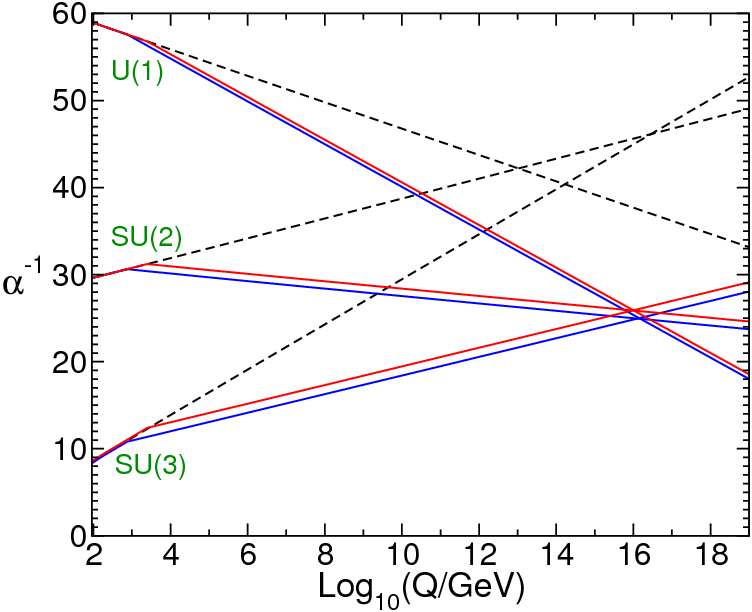
\includegraphics[width=\textwidth]{images/gauge_coupling_unification}
    \legend{The sparticle masses are varied between 0.5-1.5 TeV, and $\alpha_3(m_Z)$ is varied between 0.117 and 0.121.}
  \label{fig:gauge_coupling_unification}
\end{marginfigure}
\noindent The minimal phenomenologically viable incorporation of supersymmetry into the Standard Model is known as the \emph{Minimal Supersymmetric Standard Model}, or the MSSM. Although the hierarchy problem has been the main driving force behind the development of supersymmetry, there are other motivations to study it as well.
One of them is that it has the right particle content to unify the strong and electroweak couplings at a high energy scale, as seen in \autoref{fig:gauge_coupling_unification}.

The third major motivation (and the one most relevant to this dissertation) is the fact that the MSSM contains a viable dark matter candidate. The theory admits a new kind of discrete symmetry known as \emph{R-parity}, which is an analogue of baryon and lepton number conservation. The Lagrangian of the MSSM is defined to be invariant under the action of the operator $P_R$, with eigenvalues $(-1)^{3(B-L)+2s}$, where \emph{B, L}, and \emph{s} represent the baryon number, lepton number, and spin of the field that is acted upon, respectively. As a consequence of this symmetry, the lightest supersymmetric particle (LSP) cannot decay further into other particles, thus making it a good candidate for dark matter.

\subsection{The supersymmetry algebra}
In 1967, Coleman and Mandula \citep{Coleman:1967ad} showed that, given certain assumptions, the only possible Lie group symmetries allowed for relativistic interacting field theories in four dimensions are direct products of the Poincar\'e group and an internal symmetry group (i.e. a gauge symmetry) \citep{Mandula:2015}.
A Lie algebra is defined by the commutation relations of its generators. If we extend the notion of a Lie algebra to include \emph{anticommutation} relations \citep{Wess:1974tw}, this restriction no longer applies. These kinds of algebras are known as \emph{graded Lie algebras}, or \emph{superalgebras}. The trio of Haag, Łopuszanski, and Sohnius \citep{Haag:1974qh} applied a similar treatment as Coleman and Mandula to determine the most general superalgebra consistent with relativistic quantum field theory. The generators $Q_\alpha$ of this algebra are known as fermionic operators, and must transform as Weyl spinors. The anticommutation (and commutation) relations take the form
\sidepar{The supersymmetry algebra}
\begin{align}
  \begin{split}
  \{Q_\alpha, \bar{Q}_{\dot{\beta}}\} &= 2(\sigma^\mu)_{\alpha\dot{\beta}}P^\mu\\
  \{Q_\alpha, Q_\beta\} &= \{\bar{Q}_{\dot{\alpha}}, \bar{Q}_{\dot{\beta}}\} = 0\\
  [P^\mu,Q_\alpha] &= [P^\mu,\bar{Q}_{\dot{\alpha}}] = 0
\end{split}
\label{eq:susy_algebra}
\end{align}
where $P_\mu = i\partial_\mu$ is the generator of translations. 

The first supersymmetric Lagrangian density in four-dimensions was formulated by Wess and Zumino \citep{Wess:1974tw}. The approach taken was to define infinitesimal `supergauge' transformations for scalars and spinors that generated a closed algebraic structure. Soon afterwards, Salam and Strathdee \citep{Salam:1974yz} created a more systematic approach to constructing these transformations, by giving them a geometric interpretation. 

In this picture, supersymmetric transformations can be viewed as translations in a manifold known as \emph{superspace}, which is obtained by adding the `fermionic' coordinates $\theta^\alpha$ and $\bar{\theta}^{\dot{\beta}}$ to the regular `bosonic' spacetime coordinates $x^\mu$. 
\sidepar{Generators of superspace translations}
The generators of these translations are represented by
\begin{align}
  Q_\alpha &= \frac{\partial}{\partial\theta^\alpha}-i(\sigma^\mu \bar{\theta})_\alpha \partial_\mu&&\text{and}&&
  \bar{Q}_{\dot{\beta}} = \frac{\partial}{\partial\bar{\theta}^{\dot{\beta}}}-i(\sigma^\mu\bar{\theta})_{\dot{\beta}}\partial_\mu.
\label{eq:susy_operators_diff_form}
\end{align}
These transformations act on objects known as superfields, which are complex scalar fields parameterized by the coordinates $(x^\mu,\theta,\bar{\theta})$.
Under an infinitesimal supersymmetry transformation, a general superfield $S(x,\theta,\bar{\theta})$ transforms as
\begin{align}
S\rightarrow S' = (1+i\xi^\alpha Q_\alpha + i\bar{\xi}_{\dot{\alpha}}\bar{Q}^{\dot{\alpha}})S
\label{eq:gen_susy_transformation}
\end{align}
where $\xi^\alpha$ and $\bar{\xi}_{\dot{\alpha}}$ are two-component Weyl spinor fields that parameterize the translation.
The fermionic coordinates $\theta$ and $\bar{\theta}$ each have two components. For example, $\theta$ can be represented as $\theta^\alpha = (\theta^1,\theta^2)$. Each of these two components is a \emph{Grassmannian} variable, satisfying the anticommutation relation $\{\theta^i,\theta^i\} = 0$. This implies that $(\theta^i)^2 = 0$. This means that a Taylor expansion in powers of a fermionic coordinate must always terminate with a finite number of terms. For a general superfield \emph{S}, the Taylor expansion about the fermionic coordinates $\theta,\bar{\theta}$ takes the form
\sidepar{General superfield expansion}
\begin{align}
  \begin{split}
  S(x,\theta,\bar{\theta}) = a &+ \theta\xi + \bar{\theta}\chi^\dagger + \theta\theta b + \bar{\theta}\bar{\theta}c+\bar{\theta}\bar{\sigma}^\mu\theta v_\mu \\
  &+ \bar{\theta}\bar{\theta}\theta\eta + \theta\theta\bar{\theta}\zeta^\dagger+\theta\theta\bar{\theta}\bar{\theta}d,
\end{split}
  \label{eq:general_superfield_expansion}
\end{align}
where \emph{a,b,c} and \emph{d} are complex-valued scalar fields, $\xi,\chi,\eta$ and $\zeta$ are spinor fields, and $v_\mu$ is a vector field. These coefficients in the Taylor expansion will be identified with the regular (non-super) fields that we see in the SM and its supersymmetrized version, the MSSM. The matter content of the MSSM can be derived from expanding superfields of a particular type, known as \emph{chiral} superfields, with mass dimension 1. The expansion of a generic chiral superfield $\Phi$ takes the form:
\sidepar{Chiral superfield expansion}
\begin{align}
  \begin{split}
  \Phi(y,\theta) &= \phi(x) + \sqrt{2}\theta\psi(x)+\theta\theta F(x)\\
  &+i\theta\sigma\bar{\theta}\partial_\mu\phi(x)-\frac{1}{2}\theta\sigma\bar{\theta}\theta\sigma^\nu\bar{\theta}\partial_\mu\partial_\nu\phi(x) + \sqrt{2}\theta i\theta\sigma\bar{\theta}\partial_\mu\psi(x)
\end{split}
  \label{eq:chiral_superfield_expansion}
\end{align}
Similarly the gauge bosons come from the expansion of dimension-0 \emph{vector} superfields $V$, obtained by imposing the condition $V = V^\dagger$. 
\sidepar{Vector superfield expansion}
The expansion of $V$ takes the form:
\begin{align}
V = \bar{\theta}\bar{\sigma}^\mu\theta A_\mu+\bar{\theta}\bar{\theta}\theta\lambda+\theta\theta\bar{\theta}\lambda^\dagger+\frac{1}{2}\theta\theta\bar{\theta}\bar{\theta}D.
\label{eq:vector_superfield_expansion}
\end{align}
We see that the expansion of the chiral superfield $\Phi$ contains a scalar field $\phi$, a Weyl fermion $\psi$, and a field $F$. Thus, choosing values of $\phi,\psi$, and $F$ fixes $\Phi$. These fields, known as the \emph{component fields} of $\Phi$ can be naturally placed in a collection known as a \emph{supermultiplet}. The scalar superpartners $\phi$ are referred to as \emph{sfermions}. 
Similarly, the vector field $A_\mu$, the fermion field $\lambda$, and the field \emph{D} form another natural grouping, called a \emph{vector} supermultiplet. The fields $A_\mu$ and $\lambda$ are superpartners of each other, and fields such as $\lambda$ are generically known as \emph{gauginos}. The particle content of the MSSM, grouped into supermultiplets, is shown in tables \ref{tab:chiral_supermultiplets} and \ref{tab:gauge_supermultiplets}. For brevity, we have not shown all three fermion generations. Also, the fields $F$ and $D$ are not included, since they are \emph{auxiliary} fields, serving only to make sure that supersymmetry holds off-shell. The gauge structure of the MSSM is the same as that of the SM - there are no new gauge interactions.

The mass terms and Yukawa terms of the MSSM Lagrangian come from the collection of terms known as the \emph{superpotential}. 
\sidepar{The MSSM superpotential}
In terms of the chiral superfields in \autoref{tab:chiral_supermultiplets}, we can write the MSSM superpotential as:
\[W_\text{MSSM} = \overline{u}\mathbf{y_u}QH_u-\overline{d}\mathbf{y_d}Q H_d-\overline{e}\mathbf{y_e}L H_d+\mu H_u H_d \]
Here, we have abbreviated terms such as $\mu(H_u)_\alpha (H_d)_\beta\epsilon^{\alpha\beta}$ to $\mu H_u H_d$. The matrices $\mathbf{y}$ are $3\times3$ matrices of Yukawa couplings, with indices corresponding to the three generations of fermions. Note also that we now see the necessity of having two Higgs doublets - one that couples to the up-type fermions, and the other to the down-type fermions. A term like $\overline{u}\mathbf{y_u}QH_d^*$ would lead to a non-conserved hypercharge.

\subsection{Softly broken supersymmetry}
The component fields of a superfield have the same mass, as can be seen from expansions of the chiral and vector superfields in \eqref{eq:chiral_superfield_expansion} and \eqref{eq:vector_superfield_expansion}. This means that if supersymmetry holds, the superpartners of the SM particles should have been discovered by now. Evidently, if this symmetry exists, it is not apparent in the ground state that we inhabit - that is, it must be spontaneously broken. The exact mechanism by which it is broken is still unknown - there are a number of competing models which introduce new physics at high energy scales to spontaneously break supersymmetry. To remain model-agnostic, we can parameterize our ignorance by inserting the relevant terms into the Lagrangian by hand, with their form constrained by the requirement that the quadratic divergences in the radiative corrections to scalar masses must still vanish.

\begin{table}
  \begin{tabular}{cccccc}
    \toprule
                    & \multicolumn{2}{c}{Components}                  & \multicolumn{3}{c}{Group representation} \\ \cmidrule(r){2-3}\cmidrule(l){4-6}
    Superfield      & Spin-0                                          & Spin-$\slantfrac{1}{2}$                                                        & $SU(3)$            & $SU(2)$      & $U(1)_Y$\\\midrule
                    & Squarks                                         & Quarks                                                                         &                    &              & \\ \cmidrule(r){2-3}\\
    Q               & $\vdoublet{\widetilde{u}_L}{\widetilde{d}_L}$   & $\vdoublet{u_L}{d_L}$                                                          & $\mathbf{3}$       & $\mathbf{2}$ & $\frac{1}{2}$\\\\
    $\overline{u}$  & $\tilde{u}_R^*$                                 & $u_R^\dagger$                                                                  & $\bar{\mathbf{3}}$ & $\mathbf{1}$ & -$\frac{2}{3}$\\\\
    $\overline{d}$  & $\tilde{d}_R^*$                                 & $d_R^\dagger$                                                                  & $\bar{\mathbf{3}}$ & $\mathbf{1}$ & $\frac{1}{3}$\\\\\cmidrule{2-3}
                    & Sleptons                                        & Leptons                                                                        &                    &              & \\ \cmidrule{2-3}\\
    \emph{L}        & $\vdoublet{\widetilde{\nu}_L}{\widetilde{e}_L}$ & $\vdoublet{\nu_L}{e_L}$                                                        & $\mathbf{1}$       & $\mathbf{2}$ & -$\frac{1}{2}$\\\\
    $\overline{e}$  & $\tilde{e}_R^*$                                 & $e_R^\dagger$                                                                  & $\bar{\mathbf{1}}$ & $\mathbf{1}$ & $1$\\\\\cmidrule{2-3}
                    & Higgses                                         & Higgsinos                                                                      &                    &              & \\ \cmidrule{2-3}\\
    $H_u$           & $\vdoublet{H_u^+}{H_u^0}$                       & $\vdoublet{\widetilde{H}_u^+}{\widetilde{H}_u^0}$                              & $\mathbf{1}$       & $\mathbf{2}$ & $\frac{1}{2}$\\\\
    $H_d$           & $\vdoublet{H_d^0}{H_d^-}$                       & $\vdoublet{\widetilde{H}_d^0}{\widetilde{H}_d^-}$                              & $\mathbf{1}$       & $\mathbf{2}$ & -$\frac{1}{2}$\\\\
    \bottomrule
  \end{tabular}
  \caption{Chiral supermultiplets of the MSSM.}
  \label{tab:chiral_supermultiplets}
\end{table}

\begin{table}
  \begin{tabular}{ccccc}
    \toprule
\multicolumn{2}{c}{Components} & \multicolumn{3}{c}{Group representation} \\ \cmidrule(r){1-2}\cmidrule(l){3-5}
Spin-$\slantfrac{1}{2}$        & Spin-1                                                                         & $SU(3)$          & $SU(2)$    & $U(1)_Y$\\\midrule
Gluinos: $\widetilde{g}$       & Gluons: \emph{g}                                                               & $\mathbf{8}$       & $\mathbf{1}$ & $0$ \\\\
Winos: $\widetilde{W}^0$       & \emph{W} bosons: $W^\pm$                                                              & $\bar{\mathbf{1}}$ & $\mathbf{3}$ & $0$\\\\
Binos: $\widetilde{B}^0$       & \emph{B} bosons: $B^0$                                                                & $\bar{\mathbf{1}}$ & $\mathbf{3}$ & $0$\\
    \bottomrule
  \end{tabular}
  \caption{Gauge supermultiplets of the MSSM.}
  \label{tab:gauge_supermultiplets}
\end{table}

The soft supersymmetry breaking terms of the MSSM, written in terms of the component fields from tables \ref{tab:chiral_supermultiplets} and \ref{tab:gauge_supermultiplets} are as follows.
\sidepar{Soft supersymmetry breaking terms}
\begin{align*}
  \begin{split}
    \mathcal{L}_\text{soft}^\text{MSSM} = &-\frac{1}{2}\left(M_1\widetilde{B}\widetilde{B}+
    M_2\widetilde{W}\widetilde{W} + M_3\widetilde{g}\widetilde{g} + \text{h.c.}\right)\\
    &-\left(\widetilde{\overline{u}}\mathbf{a_u}\widetilde{Q}H_u-
    \widetilde{\overline{d}}\mathbf{a_d}\widetilde{Q}H_d-
    \widetilde{\overline{e}}\mathbf{a_e}\widetilde{L}H_d+\text{h.c.}\right)\\
    &-\widetilde{Q}^\dagger\mathbf{m}_{\widetilde{Q}}^2\widetilde{Q}
     -\widetilde{L}^\dagger\mathbf{m}_{\widetilde{L}}^2\widetilde{L}
     -\widetilde{\overline{u}}^\dagger\mathbf{m}_{\widetilde{\overline{u}}}^2\widetilde{\overline{u}}^\dagger
     -\widetilde{\overline{d}}^\dagger\mathbf{m}_{\widetilde{\overline{d}}}^2\widetilde{\overline{d}}^\dagger
     -\widetilde{\overline{e}}^\dagger\mathbf{m}_{\widetilde{\overline{e}}}^2\widetilde{\overline{e}}^\dagger\\
     &-m^2_{H_u}H^*_uH_u-m^2_{H_d}H_d^*H_d-(bH_uH_d+\text{h.c.}) 
  \end{split}
  \label{eq:soft_susy_breaking_terms}
\end{align*}
The tildes denote superpartners of the corresponding SM fields. The parameters $M_1$, $M_2$, $M_3$ govern the masses of the gauginos $\widetilde{B}$, $\widetilde{W}$, and $\widetilde{g}$, respectively.

\subsection{Phenomenological approximations}
The MSSM has a number of simplifying assumptions motivated both by calculational convenience and compatibility with observed experimental data. For example, it is convenient to take the Yukawa matrices $\mathbf{y_u,y_d,y_e}$ in a simplified limit, where only the heaviest generations have non-zero Yukawa couplings:
\begin{align*}
  \mathbf{y_u} \approx \begin{pmatrix}
    0 & 0 & 0\\
    0 & 0 & 0\\
    0 & 0 & y_t
  \end{pmatrix},&&
  \mathbf{y_d} \approx \begin{pmatrix}
    0 & 0 & 0\\
    0 & 0 & 0\\
    0 & 0 & y_b
  \end{pmatrix},&&
  \mathbf{y_e} \approx \begin{pmatrix}
    0 & 0 & 0\\
    0 & 0 & 0\\
    0 & 0 & y_\tau
  \end{pmatrix}.
\end{align*}
Furthermore, to suppress excessive CP-violation and flavor-changing neutral currents in the MSSM, the following approximations are often made. First, we assume that there is minimal mixing among the sfermions:
\begin{align*}
  \mathbf{m}_{\widetilde{Q}}^2 = m_{\widetilde{Q}}^2\mathbf{1},&&
  \mathbf{m}_{\widetilde{\overline{u}}}^2 = m_{\widetilde{\overline{u}}}^2\mathbf{1},&&
  \mathbf{m}_{\widetilde{\overline{d}}}^2 = m_{\widetilde{\overline{d}}}^2\mathbf{1},&&
  \mathbf{m}_{\widetilde{\overline{e}}}^2 = m_{\widetilde{\overline{e}}}^2\mathbf{1},&&
  \mathbf{m}_{\widetilde{L}}^2 = m_{\widetilde{L}}^2\mathbf{1}\\
\end{align*}
We also suppress the cubic scalar couplings of the first two families of sfermions by imposing the conditions: 
\begin{align*}
  \mathbf{a_u} = A_{u0}\mathbf{y_u},&&
  \mathbf{a_d} = A_{d0}\mathbf{y_d},&&
  \mathbf{a_e} = A_{e0}\mathbf{y_e}.\\
\end{align*}
Finally, requiring that the soft SUSY breaking parameters are real enables us to suppress excessive amounts of CP violation:
\begin{align*}
  \text{Im}(M_1)=
  \text{Im}(M_2)=
  \text{Im}(M_3)=
  \text{Im}(A_{u0})=
  \text{Im}(A_{d0})=
  \text{Im}(A_{e0})=0.
\end{align*}
With the above ingredients, one can work out myriad phenomenological consequences. In \autoref{ch:DM_100_TeV}, we examine the neutralino sector of the MSSM in slightly more detail, and present an analysis aimed at exploring it at a 100 TeV collider.
